\tikzset{
		>=stealth',
	    %BASE STYLE
	    base/.style = {minimum height=0.1cm,
	                   minimum width=0.2cm,
	                   text centered,
	                   font=\sffamily},
	    %ROUNDED STYLE
	    rounded/.style = {base,
	                      rounded corners},
}
\begin{figure}
	\centering
	\begin{tikzpicture}[scale=0.2]
		\node (Chip) {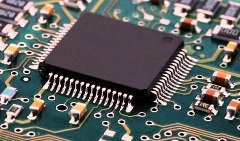
\includegraphics[width=0.1 \textwidth]{illustrations/chip}};
		\node[right = of Chip] (Scope) {
\includegraphics[width=0.1 \textwidth]{illustrations/scope}};
		\node[above right = of Chip] (PC) {
\includegraphics[width=0.1 \textwidth]{illustrations/pc}};
		\node[right = of Scope] (Trace) {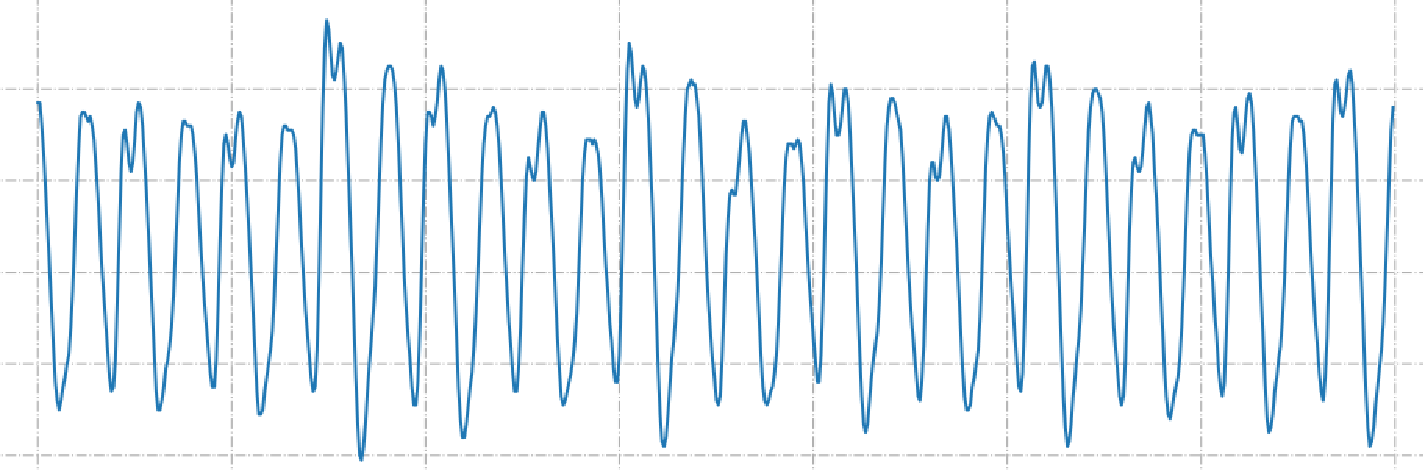
\includegraphics[width=0.2 \textwidth,angle=90]{illustrations/trace}\(\xxx\)};
		\node[rounded, fill=ceablue!30, right = of Trace] (Model) {\small \(\MLmodel(\xxx, \MLparam)\)};
		\node[right = of Model] (Scores) {
\includegraphics[width=0.2 \textwidth,angle=90]{illustrations/scores}};
		\node[rounded, fill=ceared!30, below = of Model] (Param) {\small Parameters \(\MLparam\)};
		\node[rounded, fill=ceadarkred!30, right = of PC] (Z) {\small \(\z = \miniEncrypt{\p, \keyTest}\)};


		\node[rounded, fill=cealime!30, right = of Scores] (Loss) {\small \(\lossFunc{\vNNOutput, \z}\)};

		\draw[->] (Chip)  -- (Scope);
		\draw[->] (Chip)  -- (PC);
		\draw[->] (Scope) -- (Trace);
		\draw[->] (PC)    -- (Z);
		\draw[->] (Trace) -- (Model);
		\draw[->] (Param) -- (Model);
		\draw[->] (Model) -- (Scores);

		\draw[->] (Scores) -- (Loss);
		\draw[->] (Z) -| (Loss);
		\draw[->] (Loss) |- (Param);
	\end{tikzpicture}
	\caption{Illustration of the workflow of the training of a \gls{dnn} in a profiled \gls{sca} context.}
	\label{fig:schema_dnn_sgd}
\end{figure}